\chapter{Markov Chain Monte Carlo (MCMC)}


Monte Carlo methods
are methods for using
 random number generation to
sample probability distributions.
The subject of Monte Carlo methods
has many branches, as you can see 
from its Wikipedia
category list, Ref.\cite{wiki-monte-carlo}.
MCMC (Markov
Chain Monte Carlo) is just one of those
branches, albeit a major one.
Metropolis-Hastings (MH) sampling
is a very important MCMC method.
Gibbs sampling is
a special case
of MH sampling.
This chapter covers both, MH and Gibbs sampling.
It also covers a few 
other types of sampling.

Throughout this chapter,
we use $P_\rvx:S_\rvx\rarrow [0,1]$
to denote the target probability
distribution
that we wish to obtain samples from.


\section*{Inverse Cumulative Sampling}
For more info about this topic 
and some original references, 
see Ref.\cite{wiki-inv-cum}.

This
is one of the simplest
methods for obtaining
samples from a probability 
distribution $P_\rvx$,
but it
requires knowledge
of the inverse
 cumulative distribution
of $P_\rvx$, which
is often not available.

The {\bf cumulative
distribution} function
is defined by:

\beq
CUM_\rvx(x)=P(\rvx<x)=
\int_{x'<x} dx'\;P_\rvx(x')
\;.
\eeq
Note that

\beq
P_\rvx(x)=\frac{d}{dx}CUM_\rvx(x)
\;.
\eeq


\begin{figure}[h!]
$$\xymatrix{
\rvu^{(0)}\ar[d]
&\rvu^{(1)}\ar[d]
&\rvu^{(2)}\ar[d]
\\
\ul{\vecx}^{(0)}\ar[r]
&\ul{\vecx}^{(1)}\ar[r]
&\ul{\vecx}^{(2)}
}$$
\caption{bnet for Inverse Cumulative Sampling}
\label{fig-mcmc-inverse-bnet}
\end{figure}

For $t=0, 1, \ldots, T-1$, let

$\rvu^{(t)}\in [0,1]$= random variable, 
uniformly
distributed over $[0,1]$.

$\ul{\vecx}^{(t)}=[\rvx^{(t)}_i]_{i=0,1, nsam(t)-1}$
where $\rvx^{(t)}_i \in S_\rvx$ for all $i$. 
Vector of samples collected 
up to time $t$.

The transition prob matrices, printed
in blue, for  the nodes of bnet
 Fig.\ref{fig-mcmc-inverse-bnet}, are:

\beq\color{blue}
P(u^{(t)})=1
\eeq

\beq\color{blue}
P(\vecx^{(t)}|\vecx^{(t-1)}, u^{(t)})=
\delta(\;\;\;\vecx^{(t)},
[\vecx^{(t-1)}, CUM^{-1}_\rvx(u^{(t)})]
\;\;\;)
\eeq

\hrule\noindent
{\bf Motivation}

\begin{figure}[h!]
\centering
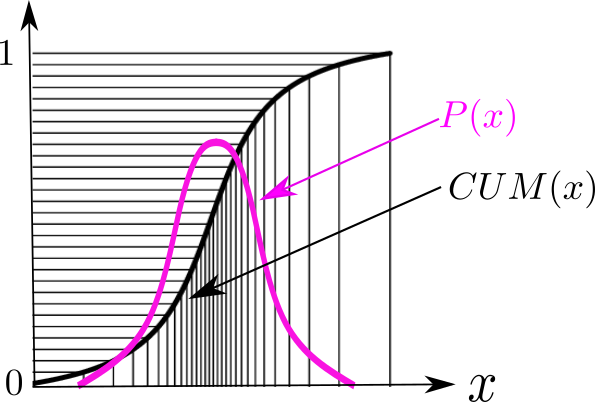
\includegraphics[width=3in]
{mcmc/inverse.png}
\caption{Motivation 
for Inverse of Cumulative Sampling.} 
\label{fig-mcmc-inverse}
\end{figure}
See Fig.\ref{fig-mcmc-inverse}.


Note that if 
$\rvu$ is uniformly distributed over 
the interval $[0,1]$ and $a\in[0,1]$, then

\beq
P(\rvu<a)=a
\;.
\eeq
Thus

\beqa
P(CUM^{-1}_\rvx(\rvu)<x)
&=&P(\rvu<CUM_\rvx(x))
\\
&=&CUM_\rvx(x)
\;.
\eeqa
Therefore,

\beq
P_\rvx(x)dx=dP(CUM^{-1}_\rvx(\rvu)<x)
\;.
\eeq


\section*{Rejection Sampling}

For more info about this topic 
and some original references, 
see Ref.\cite{wiki-reject}.

This method samples
from a ``candidates" probability distribution
$P_\rvc:S_\rvx\rarrow [0,1]$,
in cases where sampling directly
from the
target probability distribution
$P_\rvx:S_\rvx\rarrow [0,1]$
is not possible.


\begin{figure}[h!]
$$\xymatrix{
&\rvu^{(0)}\ar[d]
&&\rvu^{(1)}\ar[d]
&&\rvu^{(2)}\ar[d]
\\
\ul{\vecx}^{(0)}\ar@/^1pc/[rr]
&\rva^{(0)}\ar[r]
&
\ul{\vecx}^{(1)}\ar@/^1pc/[rr]
&\rva^{(1)}\ar[r]
&
\ul{\vecx}^{(2)}\ar@/^1pc/[rr]
&\rva^{(2)}\ar[r]
&\ul{\vecx}^{(3)}
\\
&\rvc^{(0)}\ar[u]\ar[ru]
&&\rvc^{(1)}\ar[u]\ar[ru]
&&\rvc^{(2)}\ar[u]\ar[ru]
}$$
\caption{bnet for Rejection Sampling}
\label{fig-mcmc-reject-bnet}
\end{figure}

For $t=0, 1, \ldots, T-1$, let

$\rvu^{(t)}\in [0,1]$= random variable, 
uniformly
distributed over $[0,1]$.

$\rva^{(t)}\in \bool$= accept candidate? (no=0, yes=1)

$\rvc^{(t)}\in S_\rvx$=  sample that is a 
candidate for being accepted

$\ul{\vecx}^{(t)}=
[\rvx^{(t)}_i]_{i=0,1, nsam(t)-1}$
where $\rvx^{(t)}_i \in S_\rvx$ for all $i$. 
Vector of samples collected 
up to time $t$.

This algorithm requires
 a priori definition of a candidate
probability distribution 
$P_\rvc:S_\rvx\rarrow \RR$ such that
\beq
P_\rvx(x)< \beta P_\rvc(x)
\eeq
for all $x\in S_\rvx$, for 
some $\beta\in \RR$.

The transition prob matrices, printed
in blue, for  the nodes of bnet
 Fig.\ref{fig-mcmc-reject-bnet}, are:


\beq\color{blue}
P(u^{(t)}=u)=1
\eeq

\beq\color{blue}
P(\rvc^{(t)}=c)=P_\rvc(c)
\eeq

\beq\color{blue}
P(\rva^{(t)}=a|\rvc^{(t)}=c,
\rvu^{(t)}=u)=
\left\{
\begin{array}{ll}
\delta(a, 0)&\text{ if }
u \beta P_\rvc(c)\geq P_\rvx(c)
\\
\delta(a, 1)&\text{ if }
u \beta P_\rvc(c)< P_\rvx(c)
\end{array}
\right.
\eeq

\beq\color{blue}
P(\vecx^{(t)}|
\vecx^{(t-1)}, \rva^{(t)}=a, \rvc^{(t)}=c)
=
\left\{
\begin{array}{ll}
\delta(\vecx^{(t)}, \vecx^{(t-1)})
& \text{ if $a=0$}
\\
\delta(\vecx^{(t)}, [\vecx^{(t-1)}, c])
&\text{ if $a=1$}
\end{array}
\right.
\eeq

\hrule\noindent
{\bf Motivation}

\begin{figure}[h!]
\centering
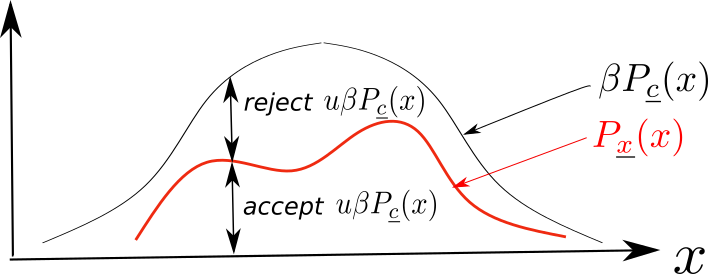
\includegraphics[width=3.5in]
{mcmc/reject.png}
\caption{Motivation 
for Rejection Sampling.} 
\label{fig-mcmc-reject}
\end{figure}
See Fig.\ref{fig-mcmc-reject}.

\section*{Metropolis-Hastings Sampling}

For more info about this topic and 
some original references, 
see Refs.\cite{bendel-metro-hast}
and \cite{wiki-metro-hast}.

An advantage of this method is that it can sample
unnormalized probability distributions
$(constant)P_\rvx$ 
because it 
only uses ratios of
$P_\rvx$ at two different points.
Another advantage
of this method
is that it scales much 
better than other sampling
methods as the number
of dimensions of the
sampled variable $\rvx$
increases.

This method produces samples that 
take a finite amount of
time to reach steady state. The samples
are also
theoretically correlated instead
of being i.i.d. as one desires.
To mitigate for the steady state problem,
one discards an initial set
of samples (the ``burn-in" period).
To mitigate for the correlation problem,
one calculates the autocorrelation
between the samples
and keeps only samples separated
by a time interval 
after which the samples 
cease to be autocorrelated to
a good approximation.



\begin{figure}[h!]
$$\xymatrix{
&\rvu^{(0)}\ar[d]
&&\rvu^{(1)}\ar[d]
&&\rvu^{(2)}\ar[d]
\\
\ul{\vecx}^{(0)}\ar@/^1pc/[rr]
&\rva^{(0)}\ar[r]
&
\ul{\vecx}^{(1)}\ar@/^1pc/[rr]\ar[rdd]
&\rva^{(1)}\ar[r]
&
\ul{\vecx}^{(2)}\ar@/^1pc/[rr]\ar[rdd]
&\rva^{(2)}\ar[r]
&\ul{\vecx}^{(3)}
\\
&\rvc^{(0)}\ar[u]\ar[ru]
&&\rvc^{(1)}\ar[u]\ar[ru]
&&\rvc^{(2)}\ar[u]\ar[ru]
\\
&\rvm^{(0)}\ar[u]\ar@/^1pc/[uu]
&&\rvm^{(1)}\ar[u]\ar@/^1pc/[uu]
&&\rvm^{(2)}\ar[u]\ar@/^1pc/[uu]
}$$
\caption{bnet for Metropolis-Hastings Sampling}
\label{fig-mcmc-metro-bnet}
\end{figure}

For $t=0, 1, \dots, T-1$, let

$\rvu^{(t)}\in [0,1]$= random variable,
uniformly
distributed over $[0,1]$.

$\rva^{(t)}\in \bool$= accept candidate? (no=0, yes=1)

$\rvc^{(t)}\in S_\rvx$= sample that is a 
candidate for being accepted

$\rvm^{(t)}\in S_\rvx$= memory
of last accepted sample

$\ul{\vecx}^{(t)}=[\rvx^{(t)}_i]_{i=0,1, nsam(t)-1}$
where $\rvx^{(t)}_i \in S_\rvx$ for all $i$. 
Vector of samples collected 
up to time $t$.

A {\bf proposal transition prob matrix} 
$P_{\rvc|\rvx}:S_\rvx^2\rarrow [0,1]$ 
must be specified a priori 
for this algorithm.

The transition prob matrices, printed
in blue, for  the nodes of bnet
 Fig.\ref{fig-mcmc-metro-bnet}, are:

\beq\color{blue}
P(u^{(t)}=u)=1
\eeq

\beq\color{blue}
P(\rvc^{(t)}=c|m^{(t)}=m)=P_{\rvc|\rvx}(c|m)
\eeq

\beq\color{blue}
P(\rva^{(t)}=a|\rvc^{(t)}=c,
\rvu^{(t)}=u,m^{(t)}=m)=
\left\{
\begin{array}{ll}
\delta(a, 0)&\text{ if }
u \geq \alp(c|m)
\\
\delta(a, 1)&\text{ if }
u < \alp(c|m)
\end{array}
\right.
\eeq
where the 
{\bf acceptance probability}
 $\alp$ is defined as

\beq
\alp(c|m)=\min\left(1,
\frac
{P_{\rvc|\rvx}(m|c)P_\rvx(c)} 
{P_{\rvc|\rvx}(c|m)P_\rvx(m)}
\right)
\;.
\eeq
Note that if the proposal distribution
is symmetric, then

\beq
\alp(c|m)=\min\left(1,
\frac
{P_\rvx(c)} 
{P_\rvx(m)}
\right)
\;.
\eeq

\beq\color{blue}
P(\vecx^{(t)}|
\vecx^{(t-1)}, \rva^{(t)}=a, \rvc^{(t)}=c)
=
\left\{
\begin{array}{ll}
\delta(\vecx^{(t)}, \vecx^{(t-1)})
& \text{ if $a=0$}
\\
\delta(\vecx^{(t)}, [\vecx^{(t-1)}, c])
&\text{ if $a=1$}
\end{array}
\right.
\eeq

\beq\color{blue}
P(\rvm^{(t)}=m|
\vecx^{(t)})=
\delta(m, \text{last component of }
\vecx^{(t)}
)
\;.
\eeq
This
last equation is only defined for $t>0$.
For $t=0$, the left hand side reduces to
$P(\rvm^{(0)}=m)$ which must 
be specified a priori.

\hrule\noindent
{\bf Motivation}

\begin{figure}[h!]
\centering
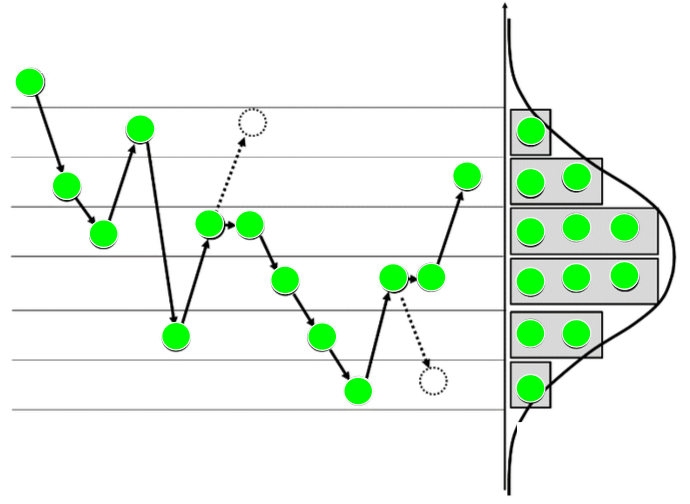
\includegraphics[width=3.5in]
{mcmc/metro-hast.png}
\caption{Motivation 
for Metropolis-Hastings Sampling.} 
\label{fig-metro-hast}
\end{figure}
See Fig.\ref{fig-metro-hast}.


Consider a time homogeneous (its
transition
matrix is the same for all times)
Markov chain with
transition prob $P(x'|x)=[T]_{x', x}$.
It's {\bf stationary distribution}, 
if it exists, is
defined as 

\beq 
\pi=\lim_{n\rarrow\infty}T^n\pi_0
\;.
\eeq

Suppose the prob distribution $P_\rvx(x)$
that we wish to sample from
satisfies

\beq
P_\rvx(x)=\pi(x)
\;.
\eeq

{\bf Reversibility (detailed balance):}
For all $x, x'\in S_\rvx$,

\beq
P(x'|x)\pi(x)=P(x|x')\pi(x')
\;.
\eeq
Detailed balance
is a sufficient (although not
necessary) condition
for a unique stationary prob
distribution $\pi$ to exist.\footnote{
As explained lucidly in 
Ref.\cite{bendel-metro-hast},
besides detailed
balance, 2 other properties
must also be satisfied
by the Markov chain,
irreducibiity
and aperiodicity. 
However,  
because of how it
is constructed, the
Metropolis-Hastings
algorithm 
automatically
produces a Markov
chain that has those
2 properties.}


Let
\beq
P(x'|x)=
P(a=1|x',x)P_{\rvc|\rvx}(x'|x)
+\delta(x,x')P(a=0|x)
\;,
\eeq
where

\beq
P(a=0|x)=\sum_{x'} P(a=0|x',x)P_{\rvc|\rvx}(x'|x)
\;.
\eeq

\begin{claim}
If

\beq
P(a=1|x',x)=\alpha(x'|x)
\;,
\eeq
then detailed balance is satisfied.
\end{claim}
\proof
Assume $x\neq x'$.

\beqa
P(x'|x)P(x)&=&
P(a=1|x',x)P_{\rvc|\rvx}(x'|x)P_\rvx(x)
\\
&=&
\min\left(1,
\frac
{P_{\rvc|\rvx}(x|x')P_\rvx(x')} 
{P_{\rvc|\rvx}(x'|x)P_\rvx(x)}
\right)
P_{\rvc|\rvx}(x'|x)P_\rvx(x)
\\
&=&
\min\left(P_{\rvc|\rvx}(x'|x)P_\rvx(x),
{P_{\rvc|\rvx}(x|x')P_\rvx(x')} 
\right)
\\
&=&
P(x|x')P(x')
\eeqa
\qed


\section*{Gibbs Sampling}
For more info about this topic and some 
original references, 
see Ref.\cite{wiki-gibbs-sam}.

Gibbs sampling is a special case
of Metropolis-Hastings sampling.
Gibbs
 sampling is ideally 
suited for application
to a bnet, because
it is stated in
terms of the conditional 
prob distributions
of $N$ random variables,
and conditional 
prob distributions are part of
the definition of a bnet.

Consider a bnet with
nodes $\rvx_0, \rvx_1, \ldots, \rvx_{N-1}$

Identify
the random
variable  $\rvx=(\rvx_0, \rvx_1, \ldots, \rvx_{N-1})$
with the
random variable  $\rvx$ used in 
Metropolis-Hastings sampling.
For Gibbs sampling,
we use the following proposal function:

\beq
P_{\rvc|\rvx}(c|m)=
\prod_{j=0}^{N-1}
P(c_j\cond [m_i]_{i\neq j})
\;.
\label{eq-gibbs-proposal}
\eeq
Eq.(\ref{eq-gibbs-proposal})
can be simplified using 
Markov Blankets
 (see Chapter \ref{ch-mblanket})
to the following:

\beq
P_{\rvc|\rvx}(c|m)=
\prod_{j=0}^{N-1}
P(c_j\cond[m_i: \forall i \ni\rvm_i\in MB(\rvc_j)])
\;,
\eeq
where for any node $\rva$,
we denote its Markov blanket by $MB(\rva)$.

\begin{figure}[h!]
$$\xymatrix{
\rvm^{(t-1)}
\ar[r]\ar[rd]\ar[rdd]\ar[rddd]
&\rvc^{(t)}_0
\ar[d]
\ar@/^2pc/[dd]
\ar@/^2pc/[ddd]
\\
&\rvc^{(t)}_1
\ar[d]
\ar@/^1pc/[dd]
\\
&\rvc^{(t)}_2
\ar[d]
\\
&\rvc^{(t)}_3
}$$
\caption{In Gibbs sampling,
the proposal distribution $P_{\rvc|\rvx}$
can be defined by making
the components $c^{(t)}_j$ of 
candidate sample $c^{(t)}$ depend on 
the previous components $(c^{(t)}_i)_{i<j}$.}
\label{fig-gibbs-candidate}
\end{figure}

An alternative proposal distribution
function that leads to much faster
convergence is as follows.
The idea is to make the components $c^{(t)}_j$ of 
candidate sample $c^{(t)}$ depend on 
the previous components $(c^{(t)}_i)_{i<j}$.
See the bnet Fig.\ref{fig-gibbs-candidate}.
The transition prob matrix for the nodes
of that bnet are


\beq\color{blue}
P(c^{(t)}_j=c_j\cond(c^{(t)}_i)_{i<j}=
(c_i)_{i<j}
,m^{(t-1)}=m)=
P(c_j|(c_i)_{i<j}, (m_i)_{i>j})
\eeq
for $j=0, 1, \ldots, N-1$. This implies

\beq
P_{\rvc|\rvx}(c^{(t)}=c|m^{(t-1)}=m)=
\prod_{j=0}^{N-1}
P(c_j|(c_i)_{i<j}, (m_i)_{i>j})
\;.
\eeq
As before, we can condition
only on the Markov blanket
of each node $\rvc_j$.

\beq
P_{\rvc|\rvx}(c^{(t)}=c|m^{(t-1)}=m)=
\prod_{j=0}^{N-1}
P(c_j|(c_i)_{i<j}, (m_i)_{i>j}, 
\text{ remove components that
are not in $MB(\rvc_j)$}
)
\;.
\eeq


\section*{Importance Sampling}

For more info about this topic and some 
original references, 
see Ref.\cite{wiki-imp-sam}.

Suppose random
variables $\rvx[s]\in S_\rvx$ for
$s=0, 1, \ldots nsam-1$ are i.i.d.
with probability distribution $P_\rvx$.
 Then
\beq
E_{\rvx}[f(x)]\approx 
\frac{1}{nsam}\sum_{s=0}^{nsam-1}
f(x[s])
\;
\eeq
for any $f:S_\rvx\rarrow \RR$.
Sometimes,
instead of using i.i.d.
samples 
$\rvx[s]\in S_\rvx$
where $\rvx[s]\sim P_\rvx$,
we wish to use i.i.d. samples
$\rvy[s]\in S_\rvx$ where
$\rvy[s]\sim P_\rvy$.


\beqa
E_\rvx[f(\rvx)]
&=&
\sum_x P_\rvx(x)f(x)
\\&=&
\sum_x P_\rvy(x))\frac{P_\rvx(x)}{P_\rvy(x)}f(x)
\\&=&
E_{\rvy}[
\frac{P_\rvx(y)}{P_\rvy(y)}f(y)
]
\eeqa

Sampling from $P_\rvy(y)$ instead
of $P_\rvx(x)$
might reduce (or increase) 
variance for a particular
 $f:S_\rvx\rarrow \RR$.

\beq
Var_\rvx[f(x)]=
E_\rvx[(f(x))^2]-(E_\rvx[f(x)])^2
\eeq

\beqa
Var_\rvy[\frac{P_\rvx(y)}{P_\rvy(y)}f(y)]&=&
E_\rvy[(\frac{P_\rvx(y)}{P_\rvy(y)}f(y))^2]-
(E_\rvy[\frac{P_\rvx(y)}{P_\rvy(y)}f(y)])^2
\\
&=&
E_\rvx[\frac{P_\rvx(x)}{P_\rvy(x)}(f(x))^2]-
(E_\rvx[f(x)])^2
\eeqa

